\section{Descripción del Sistema} \label{subsect:descripcion}
Antes de iniciar el con el desarrollo de la aplicación móvil se realizó un estudio de Tuguia.de con el objetivo familiarizarse con el contenido del sitio y el funcionamiento del API que alimenta la aplicación móvil.

\subsection{Contenido del Sitio}
El contenido de Tuguia.de es bastante variado, si bien el sitio esta planteado como una guía de locales, el portal no solo ofrece información sobre estos, también cuenta con contenido que corresponde a otro tipo de establecimientos y servicios, que van desde entidades financieras, instituciones gubernamentales, rutas de transporte, hasta  instituciones educativas. 

Los atributos relacionados con cada uno de estos \textit{nodos} de información es la siguiente: nombre, ciudad, urbanización, dirección, coordenadas geográficas, telefono de contacto, página web, correo electronico, cuenta en \textit{Facebook}, cuenta en \textit{Twitter} una o varias imagenes relacionadas, una puntuación que va del uno al cinco; esta puntuación es el resultado de promediar las calificaciones otorgadas por los usuarios en sus reseñas, por último, los nodos poseen una serie de taxonomías que permiten clasificarlos en diferentes categorías. 

Mediante la realización de peticiones de tipo HTTP en los servios provistos por el API es posible gestionar los diferentes contenidos del sitio y sus atributos.

A continuación se presenta una imagen de un Local en Tuguia.de.

\begin{figure}[h]
	\begin{center}
		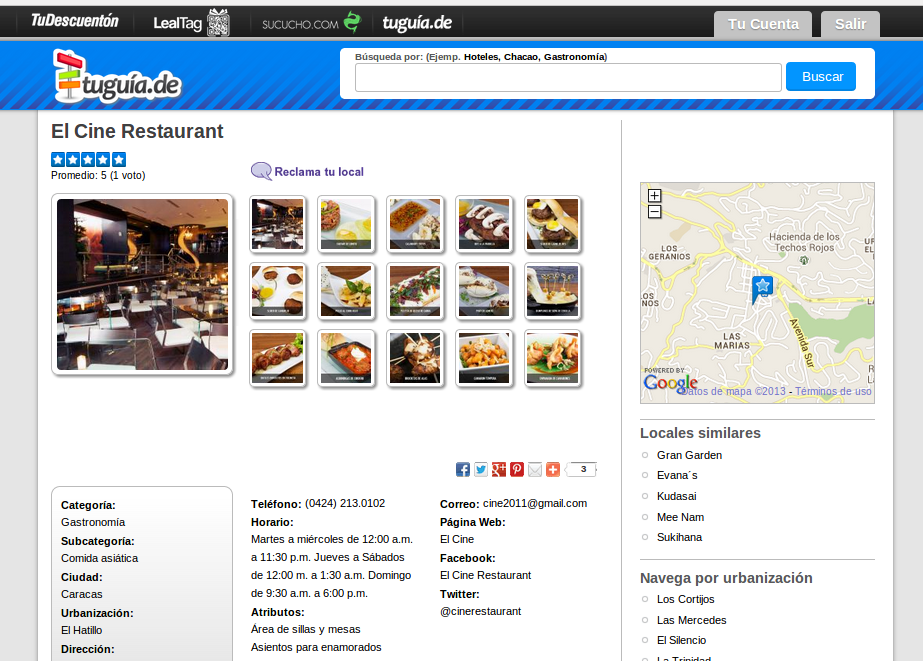
\includegraphics[scale=0.4]{imagenes/local_tgd.png}
	\end{center}
	\caption{
		\label{fig:localtgd}
		Local visto en Tuguia.de \cite{CTGD}
	}
\end{figure}


